\section{Datacenter}
Il \textbf{Datacenter} è una struttura composta da calcolatori che comunicano in rete, che aziende ed altre organizzazioni usano per organizzare, processare, memorizzare e disseminare enormi ammontare di dati. Essi rappresentano il cuore del business di un'organizzazione ed è necessario che soddisfino caratteristiche come scalabilità, sicurezza ed affidabilità oltre a possedere tutta l'attrezzatura necessaria come ad esempio la ventilazione, gruppi di continuità, sistemi di raffreddamento e naturalmente lo spazio necessario per installare il tutto. L'infrastruttura di un datacenter è cambiata molto durante gli anni e possiamo classificarla in tre categorie: 
\begin{description}
  \item[Infrastruttura Legacy:] In questa disposizione l'hardware è formato da tante commodity machines ma con l'obbligo di dover gestire ogni macchina separatamente ovvero si è costretti a dover installare su ogni macchina il sistema operativo, i programmi e le librerie necessarie. Da un primo impatto si può facilmente capire che con un numero molto grande di macchine la cosa risulta praticamente ingestibile e infatti questo modello è stato subito sostituito a favore delle architetture convergenti.
  \item[Infrastruttura Convergente:] In questa disposizione l'hardware è formato da enormi centri di calcolo che a differenza della struttura legacy sono gestiti tramite l'ausilio di un hypervisor quindi favorendo la gestione delle macchine ma con dei limiti dal punto di vista delle prestazioni in quanto la comunicazione con i dispositivi di memorizzazione avviene tramite una SAN\footnote{Storage Area Network} che rappresenta un collo di bottiglia nell'accedere e scrivere ai dati su disco.
  \item[Infrastruttura Iperconvergente:] Rappresenta la soluzione moderna per offrire un centro di calcolo performante. Questa architettura riprende il meglio delle due precedenti in quanto fa uso di commodity hardware, che costa poco, utilizza un hypervisor per gestire il datacenter ma la memorizzazione dei dati non avviene tramite una SAN. Quello che accade è che ogni rack possiede un insieme di piani che permette di aggiungere una motherboard formata da cpu, ram, e disco in modo che i dati delle singole motherboard possono accedere in maniera locale ai propri dischi aumentando le prestazioni e inoltre favorisce la scalabilità in quanto basta aggiungere al rack nuove motherboard quando è strettamente necessario.  
\end{description}
\begin{figure}[ht]
  \begin{center}
    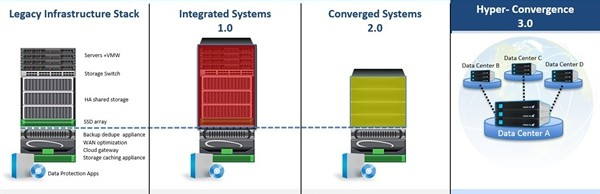
\includegraphics[width=\linewidth]{hyperconvergence.jpg}
    \caption{Le tre architetture}
    \label{hyp}
  \end{center}
\end{figure}
\section{Hypervisor}
Ogni commodity hardware che forma il moderno datacenter non si limita all'esecuzione di un unico sistema operativo in quanto questo rappresenterebbe uno spreco di risorse di memoria e di CPU che possono essede dedicate per eseguire altro calcolo. La virtualizzazione è stata la tecnologia fondamentale che ha permesso alle architetture dei datacenter di evolversi da legacy a convergenti. L'hypervisor rappresenta il componente software o hardware necessario per ottenere virtualizzazione e quando Bugnon nel 97 presentò Disco\cite{bugnon97} e il VMM (sta per virtual machine monitor ed è un sinonimo di hypervisor) nessuno avrebbe mai pensato che la sua intuizione lo avrebbe portato al successo fondando VMware.
\section{Gestione dello storage}
Essendo che un datacenter deve processare e memorizzare ordini di petabyte, quindi che non entrano in un disco commerciale, è stato necessario trovare delle soluzioni adeguate. La storia ci insegna che inizialmente i dati venivano memorizzati in enormi dischi rigidi (ricordiamo ad esempio SLED di IBM) che non solo costavano tantissimo ma occupavano tanto spazio con altezze che arrivavano addirittura a 14 pollici. La soluzione è arrivata nel 1988 grazie a Patterson e alla sua architettura \textbf{RAID} che ha evidenziato con i suoi esperimenti\cite{patterson88} che è possibile ottenere, mettendo insieme un array di dischi economici con appositi controller, più memoria, migliori prestazioni e tolleranza ai guasti.
\subsection{RAID}
L'acronimo sta per \textit{Redundant Array of Inexpensive Disks} e rappresenta l'innovazione che ha permesso di raggruppare diversi dischi dando la sensazione al sistema che possano essere utilizzati come se fossero un unico volume. L'implementazione del RAID può essere effettuata o hardware o software dove nel primo caso si usano controller hardware fatti a hoc molto costosi (più di tutti i dischi messi assieme), nel secondo caso il tutto viene gestito dal sistema operativo con un normale controller (che può essere SATA, ATI, SCSI, in fibra). Il tipo di array viene identificato dal livello RAID che determina il numero di dischi minimo necessario per poter essere configurato. La caratteristica fondamentale di questa tecnologia è quella della ridondanza che permette di individuare e correggere errori ed è ottenuta con differenti tecniche che variano a seconda del livello di RAID utilizzato:
\begin{description} 
  \item[RAID 0:]Questo livello non possiede ridondanza e utilizza lo \textbf{striping} (unità minima in cui viene diviso ogni file per la scrittura) per distribuire i file nei dischi facendo si che le letture e scritture avvengano in parallelo. Ha come svantaggio naturalmente la perdita totale dei dati in caso di rottura del disco.
  \item[RAID 1:]Questo livello fa sì che alcuni dischi vengano usati come copia per i dati in modo da intervenire in caso di guasto. Dal punto di vista delle prestazioni siamo pari a quelle di un singolo disco ma è presente la fault tolerance.
  \item[RAID 2:] Questo livello presenta delle caratteristiche simile al livello 1 ma con l'aggiunta di codici di correzione ECC dei dati. Questa configurazione è caduta in disuso a causa del fatto che ora i dischi attuali implementano di suo questa tipologia di correzione.
  \item[RAID 3:] Questo livello utilizza sia lo striping che il controllo della parità. Lo striping viene applicato a livello di segmenti e la parità mantiene le informazioni necessarie per poter recuperare i dati persi. In questo livello le scritture peggiorano poichè ad ogni scrittura si affianca il calcolo della parità e inolre la scrittura di essa avviene in un unico disco causando un collo di bottiglia sulle prestazioni totali.
  \item[RAID 4:] Questo livello utilizza le stesse funzionalità del livello 3 con la differenza che lo striping non viene effettuato con i segmenti ma a livello di blocchi.
  \item[RAID 5:] Questo livello utilizza le stesse funzionalità del livello 4 ma con la differenza che in questa configrazione non esiste un unico disco per la scrittura della parità ma su tutti vengono scritti dati o calcolo di parità (da notare che la parità non viene scritta sullo stesso disco dei dati). RAID 5 ha delle buone prestazioni che tendono a migliorare con l'aumento dei dischi installati.
  \item[RAID 6:] Questo livello ha le medesime caratteristiche del livello 5 con la differenza che effettua un doppio calcolo della parità (tramite codici di Solomon). Le prestazioni sono le medesime di RAID 5 con la presenza di una ridondanza aggiuntiva dei dati di controllo a causa della parità.
  \item[RAID Annidati:] Sono combinazioni di configurazioni di RAID permettendo così di accorpare le caratteristiche dei livelli. Le due combinazioni più diffuse sono la 01 e la 10. La prima prende due configurazioni RAID 0 e le combina in un RAID 1 e questo comporta che ogni gruppo di dischi conterrà la copia speculare dell'altro gruppo. Il secondo prende gruppi di dischi in RAID 1 e si combinano in RAID 0 permettendo così di vedere il tutto come se fosse un unico disco e inoltre permette la tolleranza del guasto di sue dischi.
\end{description}
\subsection{Software Defined Storage}
Ceph è una piattaforma di storage distribuito creata da Red Hat recentemente (2016) e rappresenta quella che potrebbe essere in futuro una valida alternativa a RAID per gestire la memorizzazione dei dati. Questa piattaforma fornisce intefacce di storage di diverse tipologie (a oggetti, a file) quindi permettendo una grande flessibilità ma soprattutto riesce a scalare nell'ordine degli exabyte. La replicazione dei dati avviene al livello software rendendo così Ceph una piattafroma indipendente dall'hardware. La ragione del suo successo risiede nel fatto che sia possibile accedere ai dati in maniera completamente trasparente e diversificata permettendo di adattarsi alle esigenze delle organizzazioni. Un'altra caratteristica a favore è che un sistema Ceph può essere costruito con commodity hardware riducendo di molto i costi a discapito di un controller RAID hardware. Ceph come molte altre realtà, rappresenta quello che oggi viene comunemente definito come \textit{Software Defined Storage} e nasce per andare incontro alle esigenze delle architetture iperconvergenti utilizzando la virtualizzazione per separare tutte le funzioni di storage dall'hardware.
\section{Sistema Operativo}
L'introduzione di tecniche efficienti per aumentare le prestazione dei dischi, non sono sufficienti per avere un datacenter efficiente. Anche il sistema operativo gioca la sua parte e deve essere implementato affinchè usi al meglio l'hardware sottostante. Questo aspetto non è da sottovalutare perchè il sistema operativo gestisce servizi cruciali come lo scheduling dei processi, gestione della memoria virtuale, mappatura dei blocchi liberi, etc... Durante la storia dell'informatica la sistemistica è stato un ambito di ricerca e sviluppo che ha sempre portanto ventate di novità questo grazie anche ad un ambiente universitario sempre competitivo e alla ricerca di nuove soluzioni che spalleggiassero la propria visione. Questo ha portato alla nascita di tantssimi sistemi, ognuno con delle caratteristiche particolari e che hanno gettato le basi per quelli moderni. Tra i più significativi è necessario citare:
\begin{description}
  \item[Tornado:] Tornado è stato uno dei primi sistemi operativi che scommise sul passaggio alle architetture multicore dei processori e si focalizzò tanissimo nello sfruttare al meglio questi ultimi massimizzandone le prestazioni sfruttando pincipi di località e tecniche di tipo Object Oriented.\cite{gamsa98}
  \item[SPIN:] SPIN è stato uno dei sistemi che ha visto nella programmazione ad oggetti un nuovo approccio per progettare sistemi operativi. Scritto completamente in un linguaggio ad alto livello come MODULA-3 vantava modularità, estensibilità senza compromettere di molto le prestazioni.\cite{bershad94}
  \item[System V:] L'unico sitema della famiglia Unix che è stato continuato ad essere sviluppato presso i laboratori AT\&T è usato tantissimo in ambito commerciale. Purtroppo il suo sviluppo è cessato nel 2003 a causa della schiacciante predominio di Windows, Linux, Mac.
  \item[BSD:] Ultimo vero superstite originario della famiglia Unix è stato uno dei primi sistemi ad includere il protocollo TCP/IP ed è famoso per la sua stabilità, affidabilità e rispetto per gli standard. In giro sono rimaste unicamente le sue controparti opensource ovvero FreeBSD e OpenBSD.
  \item[Windows NT:] Se MSDOS può non essere considerato un sistema operativo vero proprio, invece il suo successore Windows NT ha portato molti cambiamenti e Microsoft è stata una delle prime ad aggiungere il supporto ai processori Intel, in paticolare 386 e 486, intuendo da lì a poco che il mercato delle CPU si sarebbe pian piano ridotto ad un insieme ristretto di concorrenti. Questo unito alla sua semplicità ne hanno fatto il sistema operativo de facto utilizzato dall'utenza media.
  \item[Mac:] Anche Apple e Steve Jobs capirono presto che la nuova fetta di mercato su cui incentrare il nuovo business sarebbero stati i personal computer e c'era bisogno di un sistema operativo semplice ed estensibile. Codice Sorgente di BSD e il microkernel Mach messi assieme diedero vita a quello che oggi chiamiamo MacOS. Apple è stata una delle pochissime aziende big che credettero nello sviluppo di un microkernel e questa scelta le diede ragione però solo dopo tanti anni dal passaggio dai 32 ai 64 bit delle CPU.
  \item[Gnu/Linux:] Richard Stallman stanco della piega con cui il software proprietario stava prendendo piede decise di fondare il movimento Free-Software implementando insieme a decine di altri programmatori al mondo un sistema operativo che assomigliasse a Unix ma che fosse libero. Lo sforzo di tantissimi volontari diede luce al sistema GNU che non essendo ancora provvisto di un kernel (la loro scelta era di scrivere un microkernel ma la difficoltà nello sviluppo di quest'ultimo era molto alta) non gli permise di vedere la luce fino a quando un giovane studente finladese di nome Linus Torvalds non creò come tesi per il suo dottorato di ricerca un kernel monolitico che chiamò Linux. Fortuna volle che l'integrazione delle due parti fu molto semplice e anni di contributi da parte di tantissimi sviluppatori lo hanno reso il sistema operativo che oggi conosciamo: stabile, affidabile, robusto e praticamente compatibile con tipologia di hardware esistente. Queste sue caratteristiche lo rendono il signore incotrastato inambiente server e su piattaforma cloud.
\end{description}
Lo sviluppo però non fu solo dal punto di vista tecnico: anche dal punto vista algoritmico la scoperta di nuove soluzioni portarono al miglioramento dei sistemi operativi. Possiamo ricordare gli algoritmi di scheduling che sono stati progettati quanod computer e mainframe passarono ma monoutente a multiutente come ad esempio il \textbf{Fair-Scheduler} basato sul sistema a quotazioni e il \textbf{Lottery Scheduling} il cui funzionamento prevedeva un meccanismo simile al gioco della lotteria in cui l'utente col "biglietto vincente" poteva acquisire le risorse.
\subsection{Kernel}
Il componente fondamentale su cui si appoggia un sistema operativo è sicuramente il kernel. Esso si occupa dell'intera gestione dell'hardware fornendo dei meccanismi di base su cui si basano i servizi soprastanti del sistema. Proprio il numero di servizi di base che deve offrire il kernel è causa di un intero movimento che ha dato origine a vari approcci di tipo architetturale con cui deve essere sviluppato un kernel:
\begin{description}
  \item[Kernel Monolitico:] In un kernel di tipo monolitico, tutti i servizi del sistema operativo condividono la medesima area di memoria (ovvero tutto è all'interno del kernel space) del kernel ed eseguiti insieme ad esso. Il kernel espone i propri servizi tramite delle system call e permette un accesso performate all'hardware sottostante. Gli svantaggi possono essere di vario tipo: basta un unico errore in un modulo kernel per mandare in crash l'intero sistema, se il kernel comincia ad aumentare di dimensioni diventa troppo grande e soprattuto ingestibile da manutenere e soprattutto non sono portabili e quindi un passaggio potenziale ad una nuova architettura comporta la riscrittura di tutte le componenti.
  \item[Microkernel:] Il microkernel rappresenta come idea l'opposto di un kernel monolitico. L'idea alla base è di mantenere il kernel più piccolo possibile definendo unicamente le funzionalità fondamentali all'interno del kernel space (scheduling, gestione blocchi) e implementare all'interno dello user space gli altri servizi facendo sì che questi ultimi  interagiscano con il kernel attraverso scambio di messaggi tramite RPC. I vantaggi sono un kernel più compatto e più facile da manutenere, estendibilità ma al prezzo di un calo di prestazioni. C'è anche da sottolineare comunque che questo calo di prestazioni non è molto cospicuo come infatti hanno dimostrato gli studi su L4\cite{hartig97} e sui meccanismi di gestione della memoria virtuale\cite{rashid88,appel91}.
  \item[Kernel Ibridi:] Sono un ibrido tra un kernel monolitico e un microkernel e racchiudendo al suo interno qualche funzionalità in più di un normale microkernel.
  \item[Exokernel:] Sono un estremizzazione delle architetture kernel in cui il numero di astrazioni sull'hardware è ridotto all'osso permettendo agli sviluppatori di prendere le decisioni più appropriate e il kernel garantisce unicamente la gestione e messa in sicurezza delle risorse. Le applicazioni richiedono specifiche risorse fisiche (blocchi del disco, indirizzi di memoria) mentre il kernel assicura solo che le risorse siano disponibili e che l'applicativo abbia il diritto ad accederci.\cite{engler94}
\end{description}
\section{File System} 
In un datacenter è indispensabile avere un filesystem che sia trasparente e che nasconda all'utente che usufruisce del cluster l'effettiva locazione dei file sui dischi o di come siano memorizzati. L'informatica ha conosciuto diverse filosofie di implementazioni di filesystem su reti a partire dai primi anni 70 con l'invenzione del primo filesystem ma i primi tentativi concreti sono stati ottenuti con l'introduzione del protocollo \textbf{SMB} (Server Message Block) ed è ancora tuttora utilizzato da Windows e da Linux (Samba).
\subsection{AFS}
L'Andrew File system sviluppato negli anni 80 è stato il precursore dei moderni file system distribuiti. Sviluppato alla Carnagie Mellow, presentava un architettura client server (Venus e Vice) e vennero sviluppati diversi protitipi. L'idea di base è che il client Venus nell'atto di richiedere uno specifico file, localizza l'ubicazione del file, contatta il server Vice che contiene quel file e cominciano a comunicare dove le letture e le scritture del file venivano effettuate su copie in cache. Il primo prototipo soffriva di problemi di scalabilità e nella sua versione successiva, venne implementata un meccanismo di caching per migliorarne le prestazioni, ma non aveva un meccanismo di gestione della coerenza dei dati in cache su aggiornameni che avenivano in concorrenza ma solo durante le operazioni di apertura e chiusura di un file.
\subsection{NFS}
Un aprroccio completamente ortogonale ad AFS fu il Network File System o conosciuto come NFS, ideato dalla Sun Microsystem nel 1984. Anche NFS ha conosciuto varie versioni
\subsection{Coda}
\subsection{GFS}
